\chapter{Objectifs de l'application}
\section{Les trajets}
Les objectifs de ce projet sont multiples. D'abord il s'agit de réaliser une application mobile pour smartphone Android qui dispose des fonctionnalités suivantes:\bigskip

\begin{itemize}
  \item Enregistrement des coordonnées GPS du trajet
  \item Visualisation du trajet sur une carte 
  \item Consultation de l'historique des trajets 
  \item Suppression d'un trajet 
  \item Analyse des données pour obtenir :
  \begin{itemize}
    \item le temps du trajet
    \item la distance parcourue
    \item la vitesse moyenne en km/h
    \item l'allure en min/km (temps moyen pour parcourir un kilomètre)
  \end{itemize}
\end{itemize}\bigskip

\section{Les parcours}
Le second objectif est certainement le cœur du projet puisque c'est dans celui-ci que réside la nouveauté. Il s'agit de regrouper les trajets identiques pour pouvoir les comparer. Un parcours représente alors un ensemble de trajets qui suivent à peu de chose près la même trajectoire.\bigskip

Avec la mise en place de cette nouvelle structure de données nous pourrons extraire des statistiques intéressantes pour l'utilisateur à savoir:\bigskip

\begin{itemize}
  \item La meilleure performance sur le parcours
  \item Les différentes moyennes du parcours:
  \begin{itemize}
    \item le temps moyen
    \item la distance
    \item la vitesse moyenne
    \item l'allure moyenne
  \end{itemize}   
\end{itemize}\bigskip

Mais nous pourrons aussi comparer plusieurs trajectoires entre elles pour permettre à l'utilisateur de connaître en temps réel le retard ou l'avance qu'il possède par rapport à un autre trajet. L'utilisateur devra donc pouvoir fixer le trajet à prendre en référence pour chaque parcours. Ce trajet de référence

\section{Le diagramme de cas d'utilisation}
A partir de ces besoins, nous avons élaboré un diagramme de cas d'utilisation qui permet de visualiser globalement le comportement de l'application. Il décrit les enchaînements d'actions que les différents acteurs peuvent effectuer. Dans notre application il n'existe qu'un seul acteur: l'utilisateur.

\begin{img}
  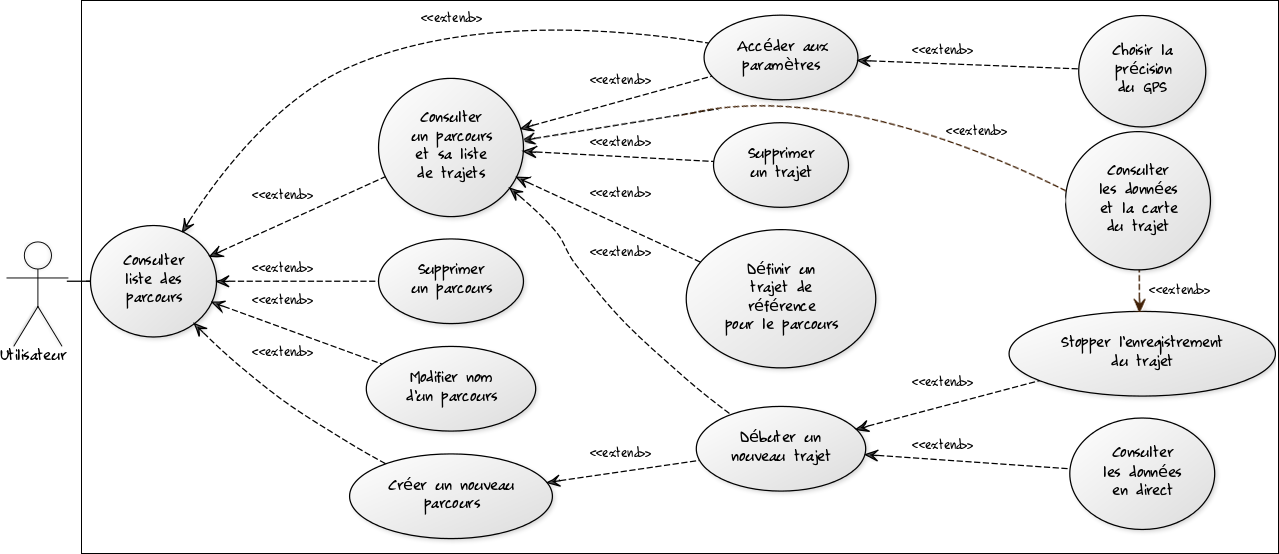
\includegraphics[scale=0.35]{img/DUC.png}
  \caption{Diagramme de cas d'utilisation de l'application}
\end{img}

\section{Les différents écrans}
Avec le diagramme de cas d'utilisation on peut facilement imaginer la structure de l'application à réaliser et le contenu des différents écrans. Quatre écrans principaux en découlent:\bigskip

\begin{itemize}
  \item La liste des parcours
  \item Le détail d'un parcours contenant sa liste de trajets
  \item Le détail d'un trajet avec l'affichage du tracé sur une carte
  \item L'écran d'enregistrement du trajet avec les données en temps réel 
\end{itemize}\bigskip

\section{Les paramètres}
On remarque un dernier cas d'utilisation nécessitant la création d'un nouvel écran, la gestion des paramètres, ou l'utilisateur pourra régler la précision du GPS. Il s'agit de définir l'intervalle d'actualisation des coordonnées GPS pour optimiser la consommation de la batterie ou la précision de son trajet. Plus la précision sera élevée, plus la consommation de la batterie sera grande et inversement.
 